\chapter{Objectives} \label{obj}

The goal of this project is the development and test of a low-cost electrical conductivity meter for liquids to be used as an aid to measure and analyze the flow in a photobioreactor.

The method chosen beforehand was to measure the fluids' electrical conductivity, which can be changed easily by adding water with differing salt concentrations. Commercially available conductivity meters are built to measure with high accuracy in order to obtain information about a liquid's absolute salinity and are relatively expensive. In our case, howeverm the meter does not need to create high-accuracy absolute measurements, but measure a relative change allowing to distinguish different liquids by their salinity. However, this needs to happen very fast and at a lot of different points in the stream. The more positions measured, the more complete the picture of the flow becomes. Therefore, the cost per sensor has to be low, to not put a restraint on the total number of points that can be measured.

The actual flow analysis is not part of this work, but rather the creation of a tool to make it possible. As such, the system needs to be designed to be easily usable by people without deep knowledge of the underlying technology.\\

The following sections describe and detail the requirements the sensor system has to fulfill in order to meet the objectives. These requirements translate the objectives into discrete and verifiable units, serving as the base for development and benchmark for the later performance analysis. 

\section{Spacial and Time Resolution}

The spacial resolution $ \diff s $ and the time resolution $ \diff t $ decide the granularity of the flow image. Both resolutions are connected by the velocity $ v $ of the stream flowing over the sensor as shown in equation \eqref{eq:resv}.

\begin{equation}
	v = \dfrac{\diff s}{\diff t}
\label{eq:resv} 
\end{equation}

With both resolutions connected, only one of them has to be defined. \\

The information gathered by the sensor has to be granular enough to enable the verification of the simulation. As it is not possible to derive a hard number from that, the following list shows different deliberations to establish a first estimate. \\

\begin{itemize}
\item The granularity of the simulation is determined by the mesh size and is in the order of about  \unit[1]{mm} to \unit[5]{mm}. A resolution better than that would be unnecessary, making this the lower limit.

\item The data collected by the sensor system shows salinity of the liquid passing a certain position over time. By extracting the same data from the simulation, a graph can be compiled comparing the measured to the simulated values. The flow becomes visible when comparing data from different positions. The first sensor to show a spike in salinity is further up the stream than sensors spiking later. The distance between two sensors has to be big enough for a given velocity of the stream so that the time delay can be clearly seen. At a flow speed of $ v $ in the order of \unitfrac[1]{m}{s}, a resolution in the order of centimeters would yield time differences of centiseconds. Whether or not this is sufficient depends on noise and delay in the sensor system, however centiseconds is a conservative estimate likely to be achievable.

\item The geometry of the inlet as shown in figure \ref{fig:elb} also influences the needed resolution. It has to be an order of magnitude smaller than the basins characteristic length, in this case the width of \unit[850]{mm}, to enable gathering data about the flow conditions within.
\end{itemize}

Derived from all that, a spacial resolution in the order of centimeters is chosen as requirement.

\begin{figure}
	\begin{center}
		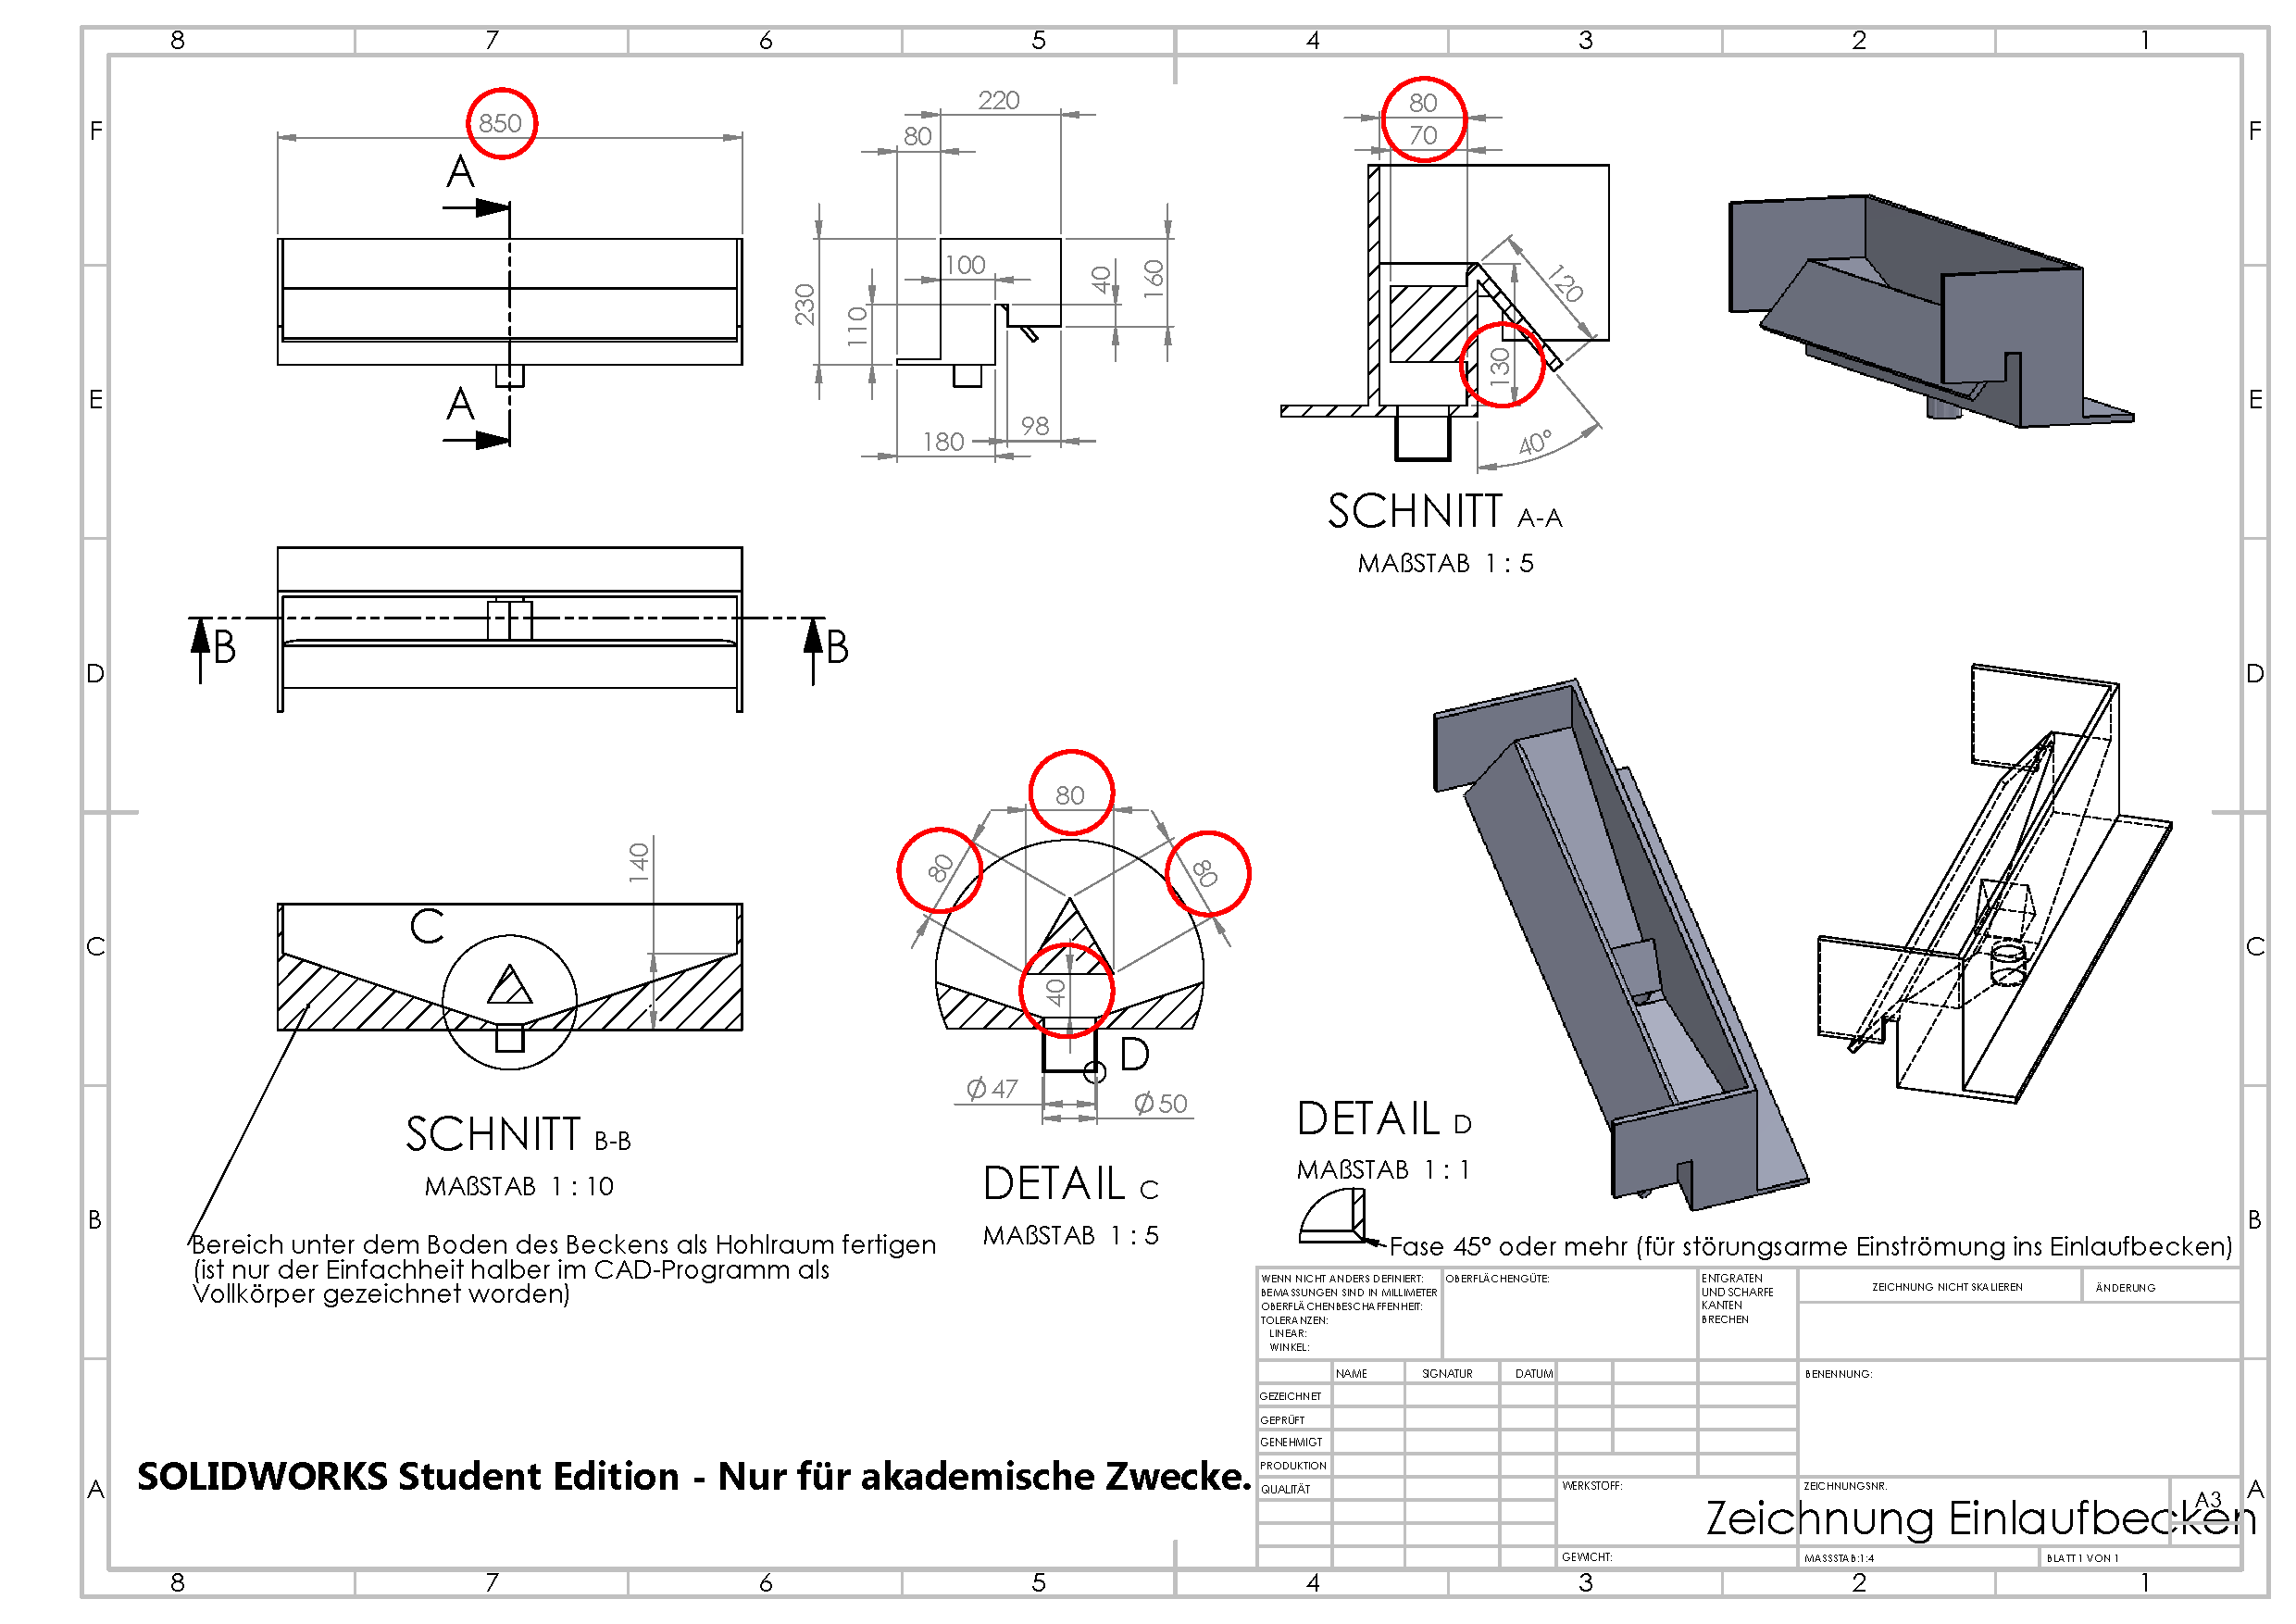
\includegraphics[width=\textwidth]{images/Einlaufbecken.pdf} 
		\caption[The inlet basin.]{The inlet basin through which the water is fed back from the bottom of the reactor to the top.}
		\label{fig:elb}
	\end{center}
\end{figure}

\section{Electrical Conductivity Resolution}

To measure the arrival of the new water stream after switching the water feed, the system has to be able to distinguish between water with different salinity. The water used normally in the reactor is tap water with a salinity of about \unit[0.2]{\%}. The salinity of the added saltwater can be chosen freely. Water with a salinity of about \unit[5]{\%} is easily available in the facilities and offers a sensible choice. Assuming a reactor with \unit[65]{l} in circulation and an added saltwater impulse of \unit[5]{l}, the resulting salinity after perfect homogenization would be approximately \unit[0.5]{\%}. The system has to be able to clearly distinguish between all those salinities. The sensors sensitivity therefore shall be better than a change of \unit[0.1]{\%} salinity with a range from 0 to \unit[5]{\%}.

\section{Cost}

The more sensors used, the more points in the stream can be measured and the better the resulting image of the stream. Therefore, the cost per sensor has to be low enough to not be prohibitive to adding more sensors.
The cost of a high quality lab conductivity meter is in the range of \euro{1000} and was set as the goal of maximum cost for the sensor system. The number of sensors needed to cover all interesting regions of the bioreactors is about 40.
A maximum cost per sensor of \euro{25} results from those figures.

\section{Usability}

The sensor system is meant to be used in the algae reactors of the algae cultivation center at the Ludwig Bölkow Campus. It has to be possible to easily mount and remove the system to and from the reactor without having to dismantle it.

The system also has to be easy to use, so it can be helpful to the researchers working on the reactor. It has to work reliably and act according to expectations of the users. The chance of handling errors that lead to loss of data has to be minimized. All operations have to be documented in a minimal set of written instructions, so the system can still be used even if the designer is not available.

\section{Requirements}

Table \ref{tab:req} concludes and displays all requirements alongside the methods of verification to be used.

\begin{table}[H]
    \centering

    \caption[Requirements]{Requirements}
    \label{tab:req}
    \begin{tabular}{lp{.7\textwidth}l}
        	\toprule
        	Nr. & Requirement & Verification \tabularnewline
        	\midrule
		1 & The system shall have a spacial resolution in the order of \unit[10]{mm}. & Test, Inspection \tabularnewline
		2 & The system shall have a sensitivity of  \unit[0.1]{\%} salinity.  & Test \tabularnewline
		3 & The system shall have a range from 0 to \unit[5]{\%} salinity.  & Test \tabularnewline
		4 & The cost per sensor shall be less than \euro{25}.  & Analysis \tabularnewline
		5 & The system shall be deployable in the algae reactor. & Demonstr. \tabularnewline
		6 & The system shall be usable with a minimal set of written instructions. & Test, Review \tabularnewline
        \bottomrule
    \end{tabular}
\end{table}